% This example An LaTeX document showing how to use the l3proj class to
% write your report. Use pdflatex and bibtex to process the file, creating 
% a PDF file as output (there is no need to use dvips when using pdflatex).

% Modified 

\documentclass{l3proj}
\begin{document}
\title{Team V - How Not To Kill Your Dog}
\author{Ross Adam \\
        Andrew Gardner \\
        Nicole Kearns \\
        Mamas Nicolaou \\
        Asset Sarsengaliyev}
\date{18 March 2013}
\maketitle

\chapter{Requirements}
\label{req}

REQUIREMENTS!

\section{Investigation Of Existing Artifacts}

\subsection{NHS Adult Drug Calculations}

The NHS Adult Drug Calculations, a smartphone based learning tool, allows the user to browse through different topics. Within each topic, there are a few slides providing the user with the information and theory, and then has ‘Check your knowledge’ slides containing multiple choice questions to see if the user has learned what that they have just read through. 

\subsection{Vet Calculator}

The Vet Calculator, an android based tool, allows the user to enter the necessary details, weight, dose, formulation, volume of fluid, etc. and the results will be provided for the user. 

\subsection{WikiVet}

\subsection{Bitesize}



\section{Client Interview}



\section{Functional Requirements}

\subsection{Requirements Table}

\textbf{Student}\\

\begin{center}
\begin{tabular}{|c|c|}
\hline \textbf{Id} & \textbf{Requirement}\\
\hline SR1 & View Topic\\
\hline SR2 & View Slides\\
\hline SR3 & View Questions\\
\hline SR4 & Answer Questions\\
\hline 
\end{tabular}
\end{center}

\textbf{User Admin}\\

\begin{center}
\begin{tabular}{|c|c|}
\hline \textbf{Id} & \textbf{Requirement}\\
\hline UAR1 & Add User\\
\hline UAR2 & Delete User\\
\hline UAR3 & Set Permissions\\
\hline 
\end{tabular}
\end{center}

\textbf{Content Admin}\\

\begin{center}
\begin{tabular}{|c|c|}
\hline \textbf{Id} & \textbf{Requirement}\\
\hline CAR1 & Add Topic\\
\hline CAR2 & Edit Topic\\
\hline CAR3 & Delete Topic\\
\hline CAR4 & Add Slide\\
\hline CAR5 & Edit Slide\\
\hline CAR6 & Delete Slide\\
\hline CAR7 & Add Questions\\
\hline CAR8 & Edit Questions\\
\hline CAR9 & Delete Questions\\
\hline 
\end{tabular}
\end{center}


\subsection{Use Case Diagrams}

\begin{center}
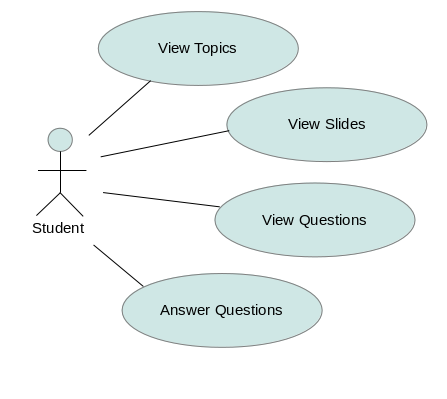
\includegraphics
[scale=0.5]
{/users/level3/0902059k/Level3/TP3/Dissertation/images/Student.png}
\end{center}
\begin{center} Student \end{center}

\begin{center}
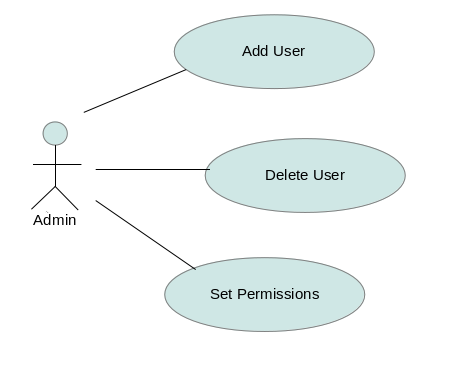
\includegraphics
[scale=0.5]
{/users/level3/0902059k/Level3/TP3/Dissertation/images/UserAdmin.png}
\end{center}
\begin{center} User Admin \end{center}

\begin{center}
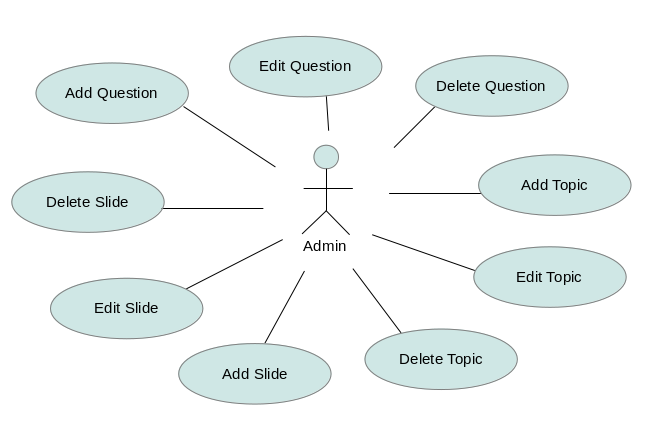
\includegraphics
[scale=0.5]
{/users/level3/0902059k/Level3/TP3/Dissertation/images/ContentAdmin.png}
\end{center}
\begin{center} Content Admin \end{center}

\subsection{Student Requirement Details}

\textbf{SR1: View Topics}\\
\textbf{Description}: Users must be able to view the different topics in the application. \\
\textbf{Rationale}: The students must be able to view the different topics in the application. This will allow them to navigate through the different topics as the progress through the slides and topics.\\
\textbf{Priority}: Must \\


\textbf{SR2: View Slides}\\
\textbf{Description}: Users must be able to view the different slides in the application. \\
\textbf{Rationale}: The students must be able to view the different slides in the learning application. The student will be able to navigate back and forward through the different slides of a topic and read through the content on each.  \\
\textbf{Priority}: Must \\


\textbf{SR3: View Questions}\\
\textbf{Description}: Users must be able to view the different questions in the application. \\
\textbf{Rationale}: The student must be able to view the questions in the application. This will allow the students to go through the different questions related to the information given in the slides.\\
\textbf{Priority}: Must\\


\textbf{SR4: Answer Questions}\\
\textbf{Description}: Users must be able to answer the questions in the application.\\
\textbf{Rationale}: The student must be able to answer the questions in the learning application. This will allow the students to test see how much they learned from the information provided in the slides. \\
\textbf{Priority}: Must\\
\textbf{Dependencies}: SR3\\


\subsection{User Admin Requirements Details}

\textbf{UAR1: Add User} \\
\textbf{Description}: \\
\textbf{Rationale}: \\
\textbf{Priority}: \\
\textbf{Dependencies}:\\

\textbf{UAR2: Delete User} \\
\textbf{Description}:\\ 
\textbf{Rationale}: \\
\textbf{Priority}: \\
\textbf{Dependencies}:\\

\textbf{UAR3: Set Permission} \\
\textbf{Description}:\\ 
\textbf{Rationale}: \\
\textbf{Priority}: \\
\textbf{Dependencies}:\\

\subsection{Content Admin Requirements Details}

\textbf{CAR1: Add Topic}\\
\textbf{Description}: \\
\textbf{Rationale}: \\
\textbf{Priority}: Must\\
\textbf{Dependencies}:\\

\textbf{CAR2: Edit Topic}\\
\textbf{Description}: \\
\textbf{Rationale}: \\
\textbf{Priority}: \\
\textbf{Dependencies}:\\

\textbf{CAR3: Delete Topic}\\
\textbf{Description}: \\
\textbf{Rationale}: \\
\textbf{Priority}: \\
\textbf{Dependencies}:\\

\textbf{CAR4: Add Slide}\\
\textbf{Description}: \\
\textbf{Rationale}: \\
\textbf{Priority}: Must\\
\textbf{Dependencies}:\\

\textbf{CAR5: Edit Slide}\\
\textbf{Description}: \\
\textbf{Rationale}: \\
\textbf{Priority}: \\
\textbf{Dependencies}:\\

\textbf{CAR6: Delete Slide}\\
\textbf{Description}:\\ 
\textbf{Rationale}: \\
\textbf{Priority}: \\
\textbf{Dependencies}:\\

\textbf{CAR7: Add Question}\\
\textbf{Description}: \\
\textbf{Rationale}: \\
\textbf{Priority}: Must\\
\textbf{Dependencies}:\\

\textbf{CAR8: Edit Question}\\
\textbf{Description}: \\
\textbf{Rationale}: \\
\textbf{Priority}: \\
\textbf{Dependencies}:\\

\textbf{CAR9: Delete Question}\\
\textbf{Description}: \\
\textbf{Rationale}: \\
\textbf{Priority}: \\
\textbf{Dependencies}:\\

\section{Non-Functional Requirements}

\end{document}
